\chapter{Fundamentos Técnicos}\label{ch:tech-reference}

\section{Hardware}

%% Descrição Meka
Para o desenvolvimento deste trabalho foi utilizado o manipulador robótico Meka A2. Sendo composto por 8 juntas com atuadores série elásticos. É um braço desenvolvido para pesquisa em tarefas em interação com pessoas de maneira segura em razão do baixo peso e da capacidade de ceder em contato com forças externas. 
Cada uma das juntas do Meka A2 utiliza um atuador elástico composto por pelo motor brushless em conjunto com uma redução baseada em engrenamento por onda de deformação, comercialmente denominado \textit{Harmonic Drive}. Este são controlados individualmente por placas DSP desenvolvidas pelo fabricante comandadas por sua vez por um computador embarcado conectado via Ethernet. Como forma de entender melhor o comportamento do robô, cada um destes componentes foi analisado de forma separada quanto as suas características de resposta no controle. Um detalhamento maior foi utilizado na descrição das ferramentas utilizadas visando facilitar a reprodutibilidade do conteúdo aqui disposto.

\begin{figure}[H]
    \centering
    \includegraphics[width=0.6\linewidth]{figs/meka.png}
    \caption{Braço Robótico Meka A2}
    \label{fig:meka_arm}
\end{figure}

\subsection{Atuadores Elásticos}

% Descrição SEA
Para garantir uma maior segurança no uso em um ambiente com pessoas são utilizados atuadores série elásticos em cada junta. Este tipo de atuador é composto pelos elementos tradicionais, motor e redução, em conjunto com algum elemento elástico entre o motor e a carga aplicada. % conforme ilustrado no diagrama ()

%% Diagrama Atuadores Elásticos

O uso de redução permite que uma alta velocidade do motor seja traduzida em um alto torque gerando uma grande inércia. Assim, quando ocorre uma colisão muita energia é transmitida ao objeto de contato bem como ao dente da engrenagem de saída, resultando internamente em um fratura no mecanismo da junta do robô. Ao se colocar um elemento elástico como uma mola, parte desta energia é absorvida e distribuída gradualmente reduzindo assim a possibilidade de fratura. De igual maneira a alta inércia representa um risco na execução de tarefas em conjunto com pessoa, pois um impacto nesta situação pode causar grande danos.

Do ponto de vista de controle, o elemento elástico atua como um filtro passa-baixa, isto é, as variações bruscas, como a colisão com algum obstáculo, são amortecidas enquanto variações baixas sofrem pouca alteração. No entanto tal acrescenta maior lentidão na resposta do sistema bem como introduz oscilações, uma vez que a energia acumulada nas molas será retransmitida gradualmente.

% https://www.cc.gatech.edu/fac/Chris.Atkeson/legs/jh1c.pdf

Em particular no meka esta forma de atuação é implementado usando um motor DC sem escova em conjunto com uma engrenagem por onda de deformação e uma placa de controle DSP. O comportamento elástico é adicionado pela próprio mecanismo de redução em conjunto com o controle de torque implementado pela placa. Desta forma a rigidez do atuador poder ser controlada via software.

\subsection{Motores Brushless}

Motores de corrente continua sem escovas ( comumente motores brusheless) são motores síncronos controlados via corrente contínua.

Tipicamente motores síncronos são controlados via corrente alternada e rotação é sincronizada com a frequência da tensão aplicada. Em um motor brushless é utilizado um inversor ou uma fonte chaveada para converter o sinal elétrico de corrente contínua em um sinal de corrente alternada com uma frequência definida. Desta forma, em conjunto com um circuito de controle interno em malha fechada, a velocidade pode ser ajustada e mantida com precisão. \cite{nobody}

\begin{figure}[H]
    \centering
    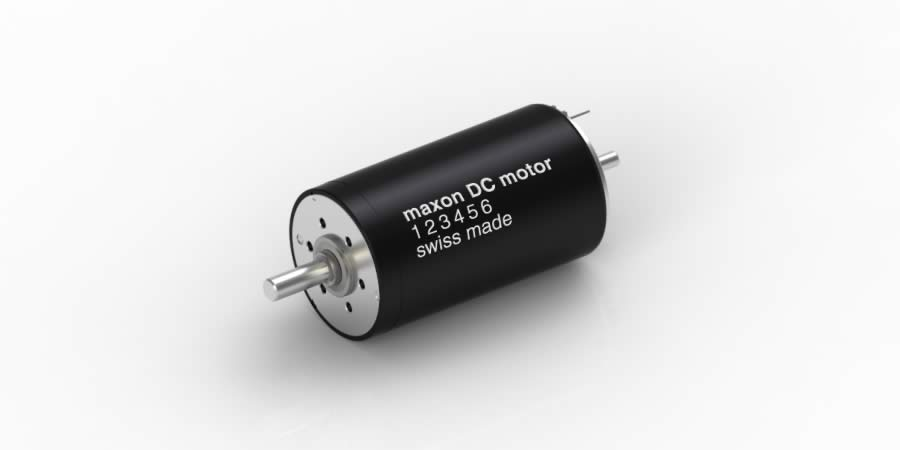
\includegraphics[width = 0.6\linewidth]{figs/maxon_servo.jpg}
    \caption{Servo Motor motor usado nas juntas do Ombro}
    \label{fig:maxon-servo}
\end{figure}

\begin{figure}[H]
    \centering
    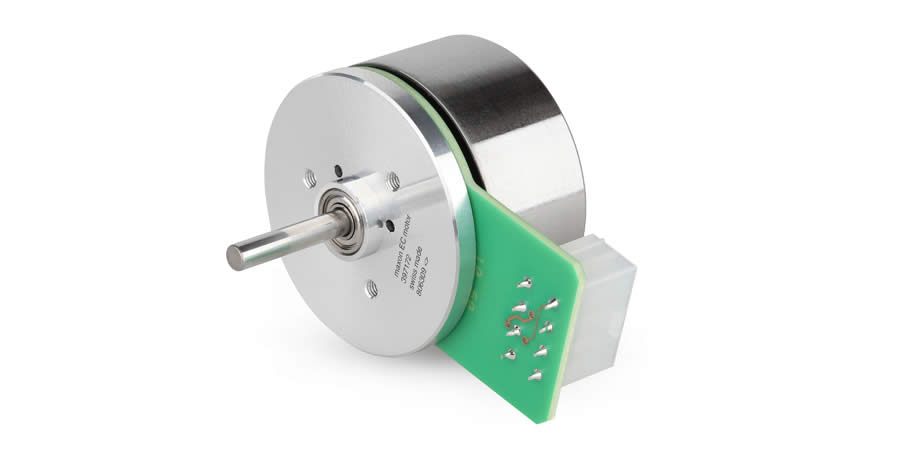
\includegraphics[width = 0.6\linewidth]{figs/maxon_flat_servo.jpg}
    \caption{Servo Motor motor usado nas demais juntas}
    \label{fig:maxon-flat-servo}
\end{figure}

% Comparativo com Motores DC
Em razão dos componentes eletrônicos usados para controle interno, motores brushless são mais caros que motores magnéticos permanentes. No entanto apresentam um custo de manutenção inferior ao

% Comparativo com Servo Motor
%% -> Servo Motor: controle de posição, torque e velocidade baseado em encoder
%% -> Motor Brushless: controle de velocidade baseado em sensor hall ( mais barato ), mais suave
% https://www.orientalmotor.com/brushless-dc-motors-gear-motors/technology/brushless-dc-motors-servo-motors-inverter.html

\subsection{Harmonic Drive}

Engrenamento por ondas de deformação, também denominado comercialmente com Harmonic drive, é um sistema mecânico para redução de velocidade baseado no deslisamento de uma membrana flexível em torno de um engrenamento.

%% Porque é necessário colocar uma redução ?
%% Gráfico Torque vs Velocidade

% Características do Motor

% https://en.wikipedia.org/wiki/Harmonic_drive
% https://en.wikipedia.org/wiki/Strain_wave_gearing
% https://en.wikipedia.org/wiki/Backlash_(engineering)

\subsection{Sensores}

Para cada junta são medidas as grandezas a posição e velocidade angular e o torque. Para tal é utilizado dois sensores: um encoder associado diretamente a junta e um sensor de corrente associado ao motor brushless. A posição de cada junta é avaliada a partir do encoder e o torque é avaliado de maneira indireta através dos sensores de corrente do motor brushless.

\begin{figure}[H]
    \centering
    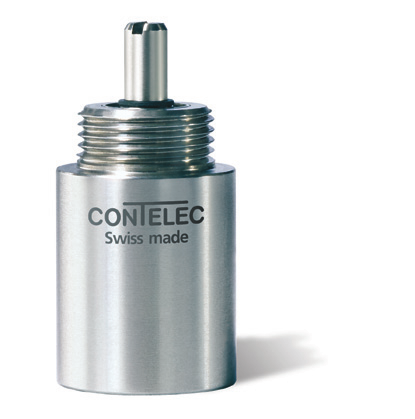
\includegraphics[width = 0.4\linewidth]{figs/vertX-encoder.png}
        \caption{Encoder utilizado nas juntas do robô}
    \label{fig:maxon-flat-servo}
\end{figure}

\subsection{DSP Control Boards}

O controle de cada junta a partir do acionamento dos motores e da leitura dos sensores é feito pela placa DSP desenvolvida pela Meka Robotics. Nela estão implementados o controle de posição, velocidade, torque e rigidez de cada atuador. Cada uma das placas possui uma interface de comunicação EtherCat ligada a um concentrador dentro do robô. Sendo este ligado através da porta Ethernet a um computador embarcado externo responsável pelo comando de cada uma das partes do robô.

\begin{figure}[H]
    \centering
    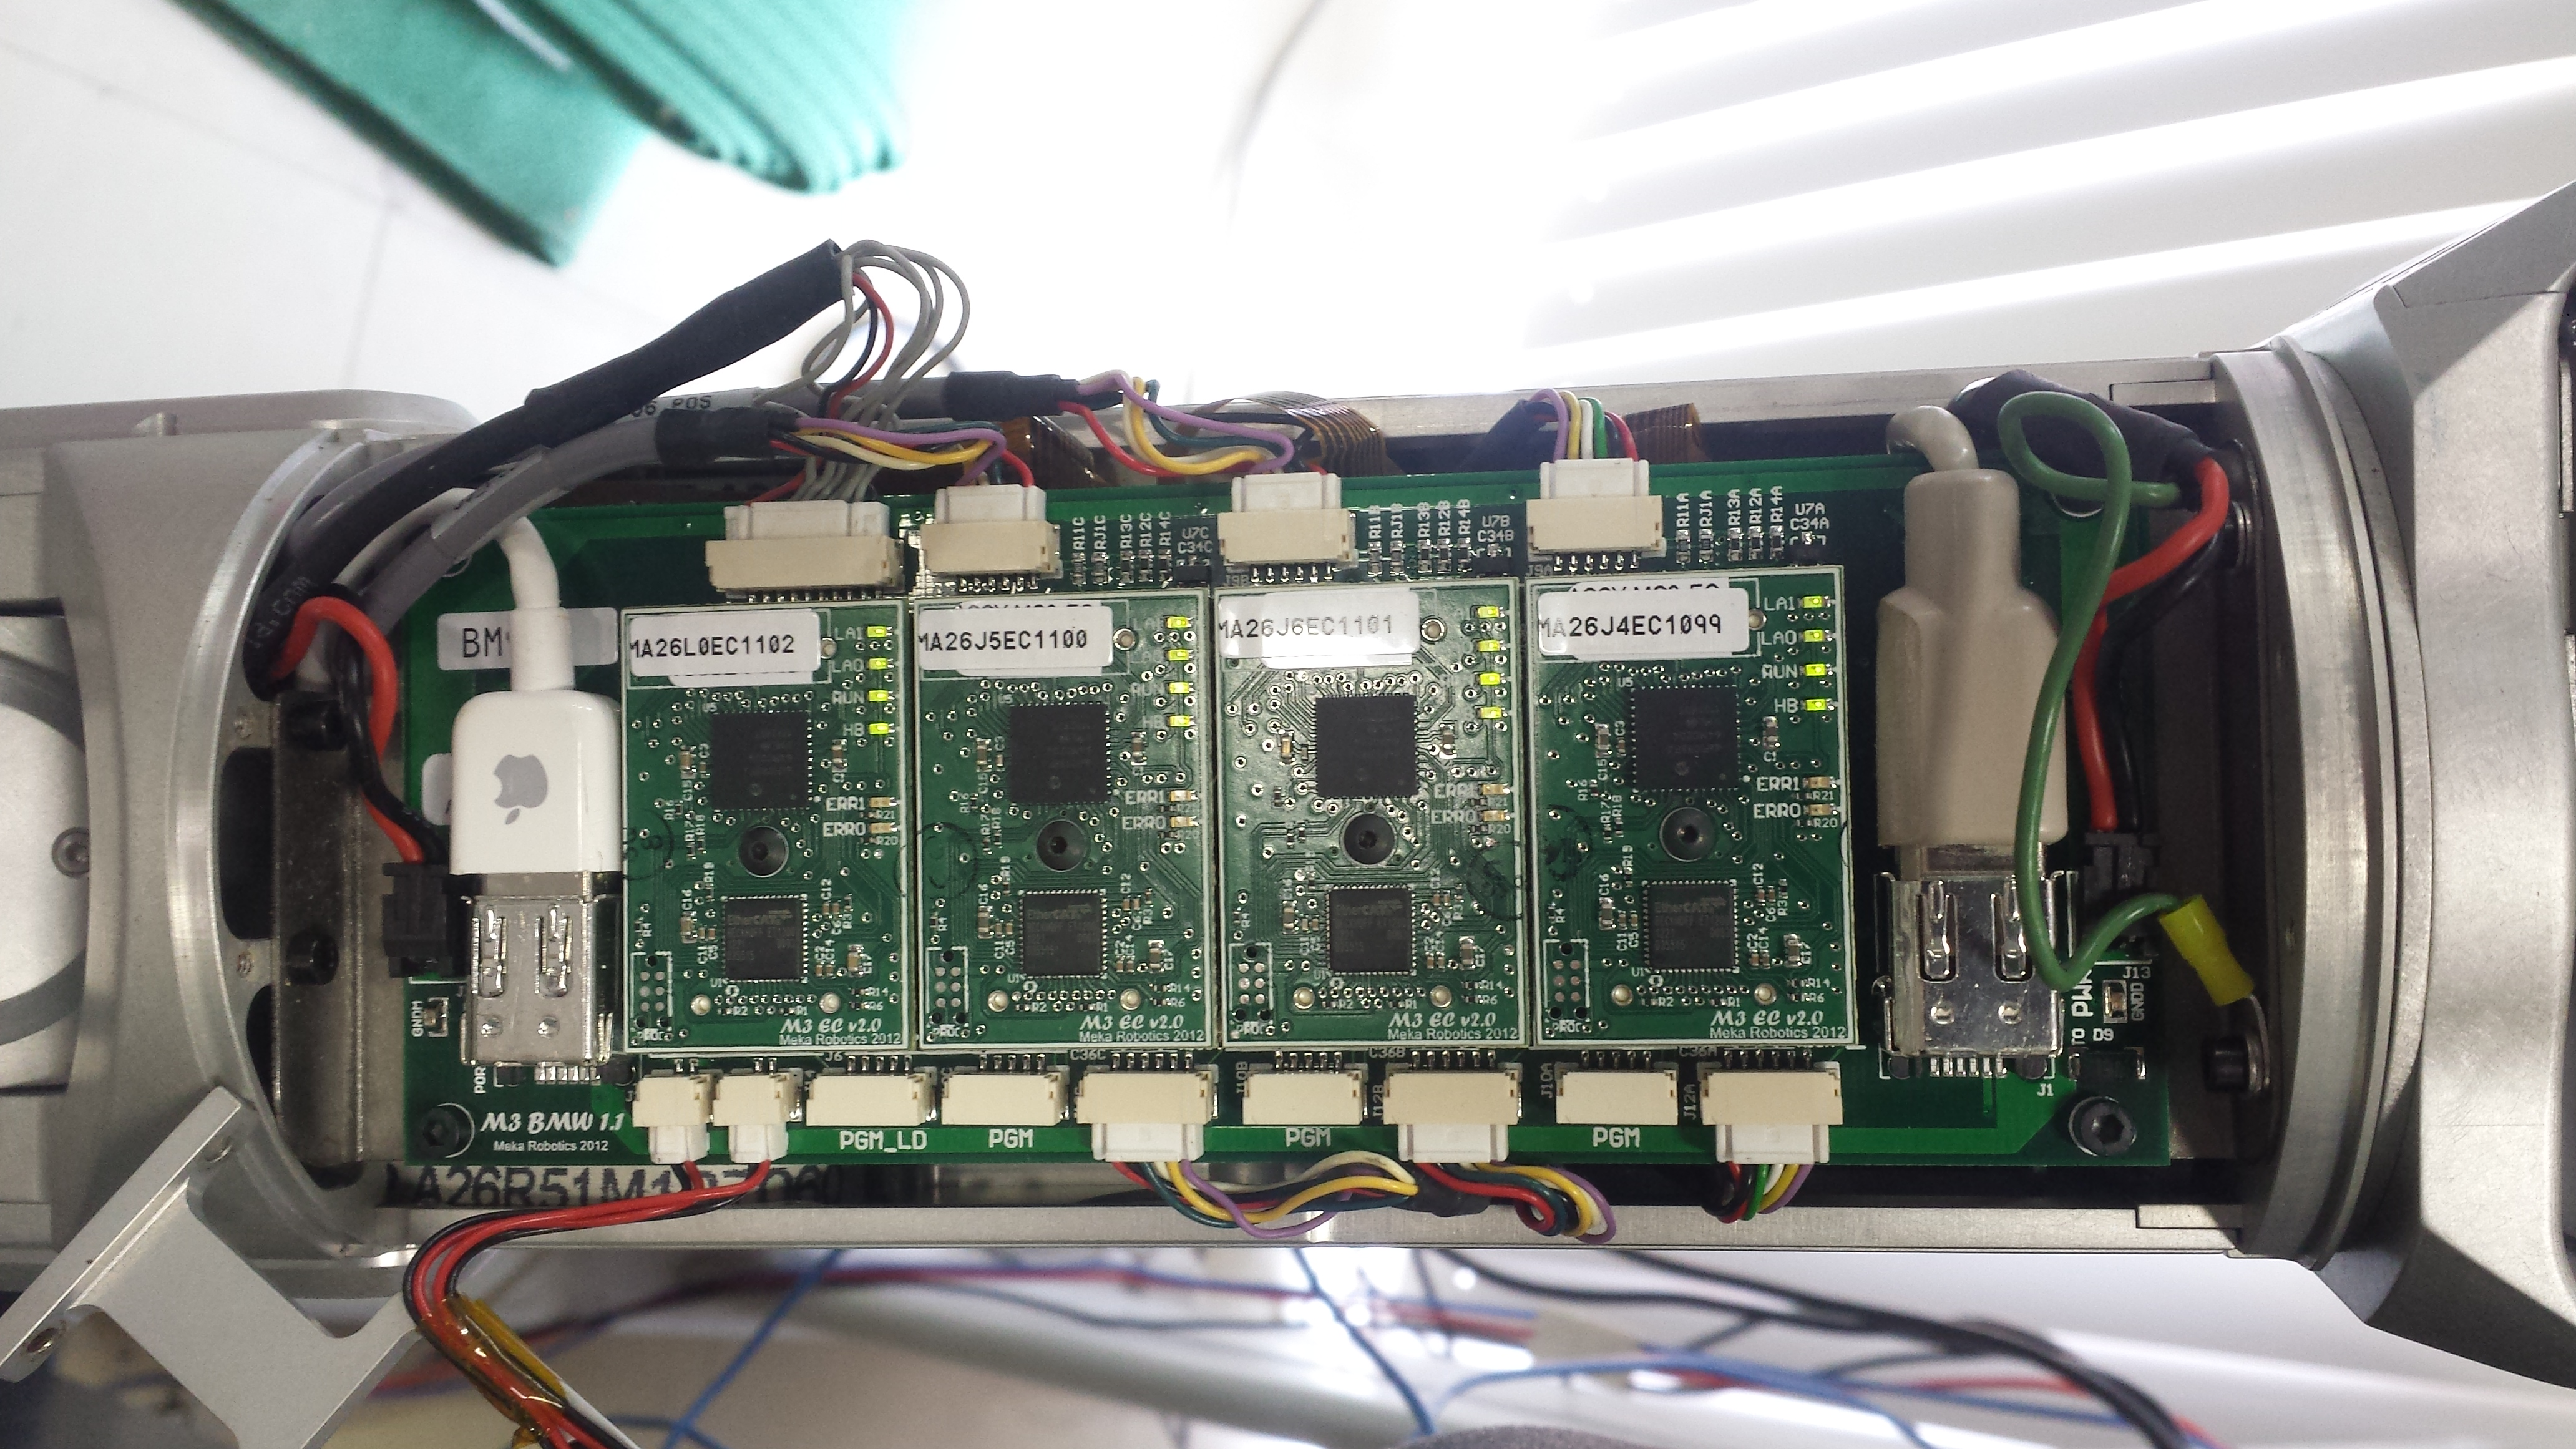
\includegraphics[width = 0.7\linewidth]{figs/dsp-control-wrist.jpg}
    \caption{Destaque Placas de controle DSP}
    \label{fig:maxon-flat-servo}
\end{figure}

\section{Software}

% Diagrama Meka

\subsection{Meka PC}

Para o controle do robô é utilizado um computador embarcado com o sistema operacional Ubuntu 12.04 e o kernel Real Time Xenomai. Nele são implementado o driver para o protocolo EtherCat e a biblioteca M3 responsável pela interação com cada um dos dispositivos, entre sensores e motores de cada junta.

Dentro do pc é executado um script que para disparar os processos relacionados a comunicação com a robô via socket pelo protocolo Ethercat e as interface para Python. Um vez que o script está em execução o robô pode ser controlado via API ou por meio de um programa para ROS, conforme ilustrado no diagrama apresentado na figura \ref{fig:m3arch}.


% m3rt_server
% -> Interface via socket
% -> Memórica compartilhada
% -> API Python
% -> ROS

\begin{figure}[ht]
    \centering
    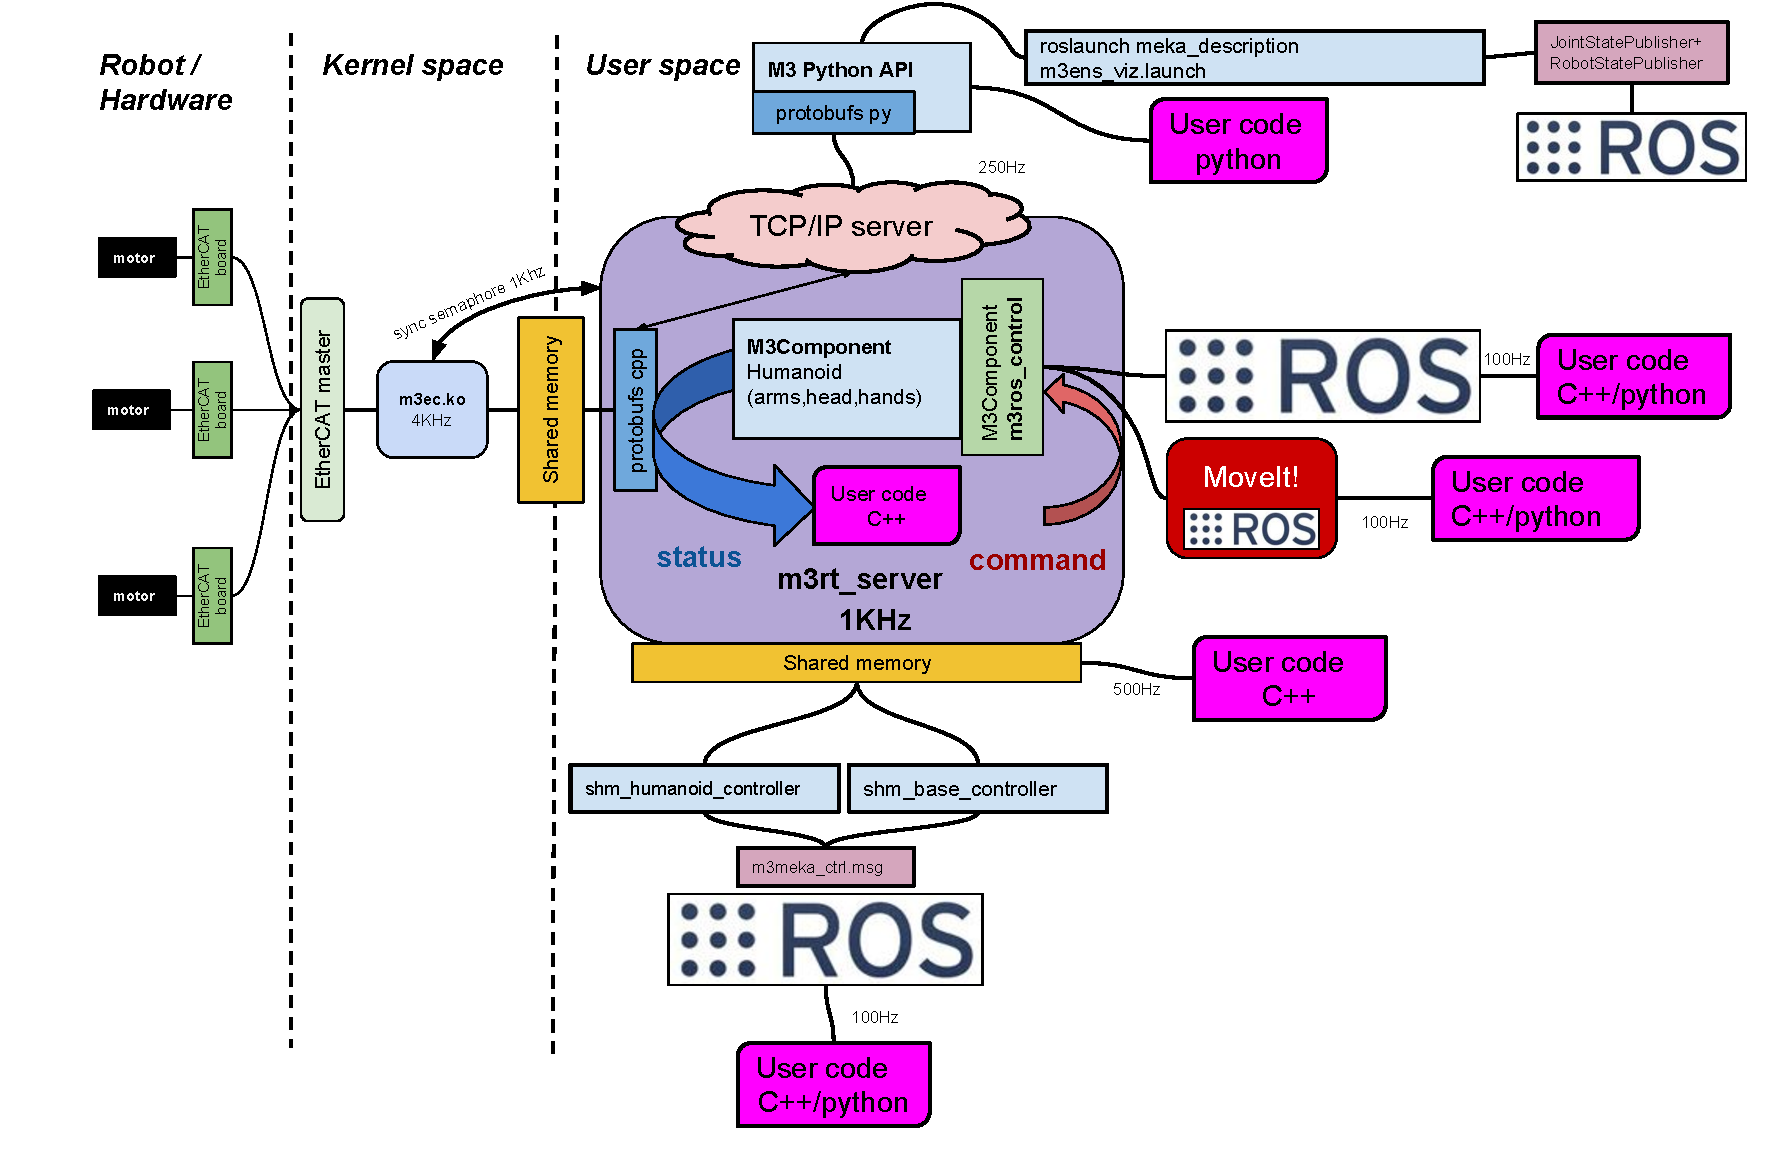
\includegraphics[width=\linewidth]{figs/m3_arch.pdf}
    \caption{Diagrama ilustrativo da arquitetura do robô}
    \label{fig:m3arch}
\end{figure}
\subsection{DQ Robotics}

A representação do robô usando quatérnions duais é feita com auxílio da biblioteca DQ Robotics. Nela estão implementados as principais operações algébricas com quartenions duais bem como alguns controladores nas liguagens Matlab, Python e C++.

\subsection{ROS}

Robotics Operating System (ROS) é um framework de software voltado para a robótica que reúne as melhores práticas para robótica em conjunto com um sistema de comunicação distribuída que permite o uso de diferentes linguagens de programação no mesmo projeto. Começou em 2007 reunindo conceitos de diversos projetos de software aberto anteriores e com o passar dos anos se tornou um padrão dentro da comunidade de robótica, contando com implementação para diversos robôs comerciais e inclusive uma versão completa voltada exclusivamente para a industria.

\subsubsection{Shm Humanoid Interface}

Este é um programa disponibilizado pela Meka Robotics para a comunicação via ROS com o Meka. O programa possui o código completamente aberto e é implementado como um nó para ROS via C++ e atua como interface entre a memória compartilhada dois tópicos no ros: /humanoid\_state e /humanoid\_command. Na versão atual são somente interpretados os comando de posição das juntas através dos modos de controle com e sem compensação da gravidade.

\subsubsection{ROS Bags}

ROS Bags é um utilitário do ROS para o registro dos eventos em cada tópico. A principal característica é que a informação pode ser lida e depois reproduzida como tópico sem a necessidade de manter o hardware conectado, permitindo a análise de diferentes experimentos diretamente pelas ferramentas do ROS.

\subsection{Python API}

Além do controle via ROS, o meka possui uma interface para Python que permite uma liberdade maior de controle uma vez que possui mais recursos já implementados. Além do modos de controle por posição estão também disponíveis o controle direto por torque e por velocidade das juntas. Estão implementados um controlador para compensação do efeito da gravidade a partir da biblioteca KDL com base no momento de inércia de cada junta.

\subsubsection{Plotly}

Plotly é uma biblioteca para gerar gráficos que porta a biblioteca D3.js para diferentes linguagens além de adicionar alguns recursos a mais. No trabalho foi utilizada para gerar os gráficos diretamente a partir do jupyter para facilitar a análise dos resultados.